\documentclass[twoside]{article}

\usepackage{epsfig}
\usepackage{float}
\usepackage{amsmath}
\setlength{\oddsidemargin}{0.25 in}
\setlength{\evensidemargin}{-0.25 in}
\setlength{\topmargin}{-0.6 in}
\setlength{\textwidth}{6.5 in}
\setlength{\textheight}{8.5 in}
\setlength{\headsep}{0.75 in}
\setlength{\parindent}{0 in}
\setlength{\parskip}{0.1 in}

\newcommand{\lecture}[3]{
   \pagestyle{myheadings}
   \thispagestyle{plain}
   \newpage
   \setcounter{page}{1}
   \noindent
   \begin{center}
   \framebox{
      \vbox{\vspace{2mm}
    \hbox to 6.28in { {\bf 10-708:~Probabilistic Graphical Models
10-708, Spring 2013 \hfill} }
       \vspace{6mm}
       \hbox to 6.28in { {\Large \hfill #1  \hfill} }
       \vspace{6mm}
       \hbox to 6.28in { {\it Lecturer: #2 \hfill Scribes: #3} }
      \vspace{2mm}}
   }
   \end{center}
   \markboth{#1}{#1}
   \vspace*{4mm}
}

\begin{document}

\lecture{Monte Carlo Methods}{Eric P. Xing}{Willie Neiswanger and Xiaohua Yan} % Lecture name, Lecturer, Scribes
\section{Introduction}
\section{Naive Sampling}
In order to draw samples from a target distribution, one intuitive is that we could directly draw different samples uniformly from the state space and evaluate $P^*(\mathbf{x})$ at these points. However, even though the samples can be easily evaluated for $P^*(\mathbf{x})$, it might still work poorly on high-dimensional distributions. To see why this is the case, consider the following \textit{alarm example}, and the table on the right displays 10 samples drawn according to the probabilities given in the BN, where 1 denotes \textit{true} and 0 denotes \textit{false}:
\begin{figure}[H]
\minipage{0.5\textwidth}
\begin{center}
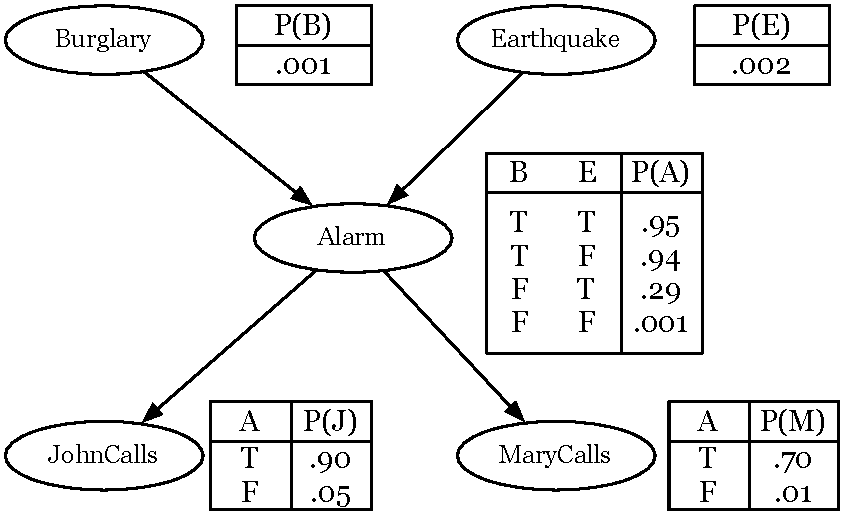
\includegraphics[scale=0.5]{alarm_example}
\end{center}
\endminipage\hfill
\minipage{0.5\textwidth}
\begin{center}
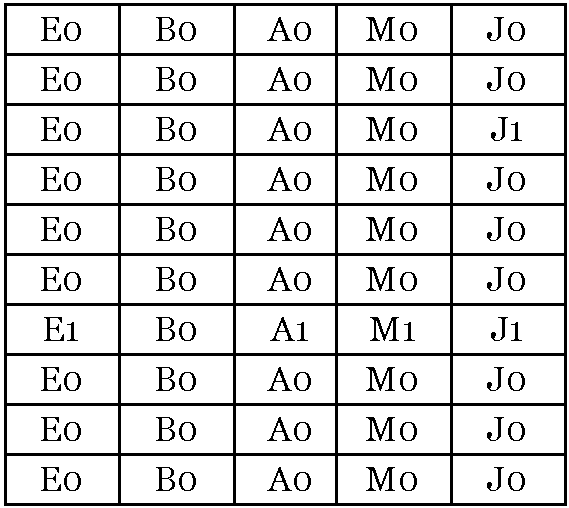
\includegraphics[scale=0.5]{alarm_table}
\end{center} 
\endminipage\hfill \\
\end{figure}
As can be observed from the example, if we want to compute $P(J|B1)$ according to the samples, the result would be $P(J|A1) = P(J,A1)/P(B1)= <0,1>$, since there is only one sample available. A more extreme case would be to compute $P(J|A1)=P(J,B1)/P(B1)$, which is not defined because there is no such sample available. Therefore, we can imagine that for a model with hundreds or more variables, rare events will be very hard to garner enough samples even after a long time of sampling.
\section{Rejection Sampling}
\section{Importance Sampling}
Importance sampling is \textit{not} a method for generating samples from the target density $P(\mathbf{x})$. Rather, it estimates the expectation of a function $\phi(x)$. Importance sampling deploys a simpler proposal distribution $Q(x)$ from which we can generate samples and satisfies the condition that $Q(x)>0$ whenever $P(x)>0$. In importance sampling, we generate $M$ samples from $Q(x)$ and suppose we can evaluate the samples for the unnormalized version of $P(x)$. For each sample, define
\[w^{(m)}=\frac{P(x^{(m)})}{Q(x^{(m)})}\]
Then the importance weighted estimator is
\begin{align*}
\hat{\Phi}(x) &=\int \phi(x)P(x)dx\\
&=\int \phi(x)\frac{P(x)}{Q(x)}Q(x)dx\\
&\simeq \frac{1}{M}\sum_m\phi(x^{(m)})\frac{P(x^{(m)})}{Q(x^{(m)})}\\
&=\frac{1}{M}\sum_m\phi(x^{(m)})w^{(m)}
\end{align*}
The unnormalized version of estimator is unbiased because we have
\[E_Q[\phi(x)w(x)]=\int \phi(x)w(x)Q(x)dx=\int \phi(x)\frac{P(x)}{Q(x)}Q(x)dx=E_P(\phi(x))\]
Suppose we can only evaluate $P^*(x)=\alpha P(x)$ instead of $P(x)$. To get around the normalization constant $\alpha$, first define
\[r(x)=\frac{P^*(x)}{Q(x)}\]
then our estimator can be derived as follows:
\begin{align*}
\hat{\Phi}(x) &= \int\phi(x)P(x)dx\\
&=\frac{1}{\alpha}\int \phi(x)\frac{P^*(x)}{Q(x)}Q(x)dx\\
&=\frac{\int \phi(x)r(x)Q(x)dx}{\int r(x)Q(x)dx}\\
&\simeq \frac{\sum_m\phi(x^{(m)})r^{(m)}}{\sum_mr^{(m)}}\\
&=\sum_m\phi(x^{(m)})w^{(m)}, \text{where } w^{(m)}=\frac{r^{(m)}}{\sum_mr^{(m)}}
\end{align*}
This importance weighted estimator is biased. For example, suppose $M=1$, then
\[E_Q[\frac{\phi(x^{(1)})r(x^{(1)})}{r(x^{(1)})}]=\int \phi(x)Q(x)dx=E_Q(\phi(x))\neq E_P(\phi(x))\]
However, the normalized importance sampling is asymptotically unbiased, and the variance of the normalized importance sampler is usually lower in practice. Also, it is common that we can evaluate $P^*(x)$ but not $P(x)$ (e.g. $P(x|e)=P^*(x)/P(e)$ for Bayes net, and $P(x)=P^*(x)/Z$ for MRF).
\section{Weighted Resampling}
\section{Rao-Blackwellised Sampling}
So far we have pointed out that sampling in high dimensional spaces can cause high variance in the estimate. The Rao-Blackwell theorem can be stated as follows:

\textbf{Rao-Blackwell Theorem:} Let $\hat{\theta}$ be an estimator, and $T$ a sufficient statistic, both for $\theta$. Then the estimator $\hat{\theta}^*(X_1,...,X_n)=E(\hat{\theta}(X_1,...,X_n)|T(X_1,...,X_n))$ is at least as good as $\theta$ in terms of mean squared errors.

Such idea can be applied to sampling. Namely, first we sample some variables $X_p$, and conditional on that, we can compute the expected value of the rest variables $X_d$ analytically:
\begin{align*}
E_{P(X|e)}[f()X] &= \int p(x_p,x_d|e)f(x_p,x_d)dx_pdx_d\\
&=\int_{x_p}p(x_p|e)\left(\int_{x_d}p(x_d|x_p,e)f(x_p,x_d)dx_d\right)dx_p\\
&=\int_{x_p}p(x_p|e)E_{p(X_d|x_p,e)}[f(x_p,X_d)]dx_p\\
&=\frac{1}{M}\sum_mE_{p(X_d|x_p^{(m)},e)}[f(x_p^{(m)},X_d)]
\end{align*}
This estimator has lower variance, because the following equation holds:
\[\text{var}[\tau(X_p,X_d)]=\text{var}[E[\tau(X_p,X_d)|X_p]]+E[\text{var}[\tau(X_p,X_d)|X_p]]\]
And hence $E[\text{var}[\tau(X_p,X_d)|X_p]]\leq\text{var}[\tau(X_p,X_d)]$.
\end{document}

